% 2013 年春季上海卷第 25 题：正三棱柱 ABC-A1B1C1
% 图中透视比例不代表题设尺寸；AC 为背面棱，画虚线。
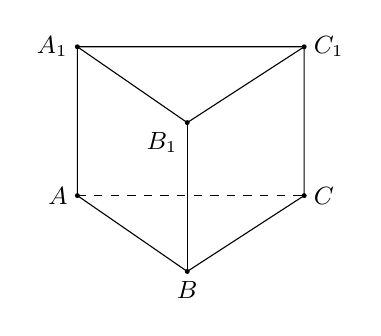
\begin{tikzpicture}[>=stealth, scale=0.9, font=\small]
  \coordinate (A)  at (0,1.45);
  \coordinate (C)  at (3.20,1.45);
  \coordinate (B)  at (1.55,0.38);
  \coordinate (A1) at (0,3.55);
  \coordinate (B1) at (1.55,2.48);
  \coordinate (C1) at (3.20,3.55);
  % 可见棱
  \draw (A1) -- (C1) -- (C) -- (B) -- (A) -- (A1);
  \draw (A1) -- (B1) -- (C1);
  \draw (B1) -- (B);
  % 不可见棱
  \draw[dashed] (A) -- (C);
  % 顶点
  \fill (A) circle (1pt) node[left] {$A$};
  \fill (B) circle (1pt) node[below] {$B$};
  \fill (C) circle (1pt) node[right] {$C$};
  \fill (A1) circle (1pt) node[left] {$A_1$};
  \fill (B1) circle (1pt) node[below left] {$B_1$};
  \fill (C1) circle (1pt) node[right] {$C_1$};
\end{tikzpicture}
